\chapter{Testing Tribler at a Large Scale}
In the previous Chapter, we performed various small performance measurements and quantified the usability and performance of common performed operations in Tribler. While these experiments gave us insights in the performance of Tribler, we focused on a single component in every experiment.\\\\
In this chapter, we focus on how the components work together. We will test Tribler on a large scale, where we start the application, perform a remote keyword search, select a download and start this download anonymously. We will first discuss the set-up of the experiment in more detail, after which we turn our focus to the results we observed during the experiment. As far as we aware, this is the first time that we assess the performance of Tribler by performing a whole 

\section{Environment Specifications}
We utilized the DAS5 supercomputer for this test at large scale. We created a separate job in our CI environment where we allocate ten nodes on the Vrije Universiteit cluster for every job execution. A summary of hardware specifications in each node is presented in Table \ref{table:das5-node-specifications}. On each node, we start exactly one Tribler session.

\begin{table}[h!]
	\centering
	\begin{tabular}{|l|l|}
		\hline
		\emph{CPU} & dual 8-core 2.4 GHz (Intel Haswell E5-2630-v3)\\ \hline
		\emph{Memory} & 64GB \\ \hline
		\emph{Hard disk} & 128TB \\ \hline
		\emph{Operating system} & CentOS Linux \\ \hline
	\end{tabular}
	\caption{The specifications of a node in the DAS5 VU cluster.}
	\label{table:das5-node-specifications}
\end{table}

\section{Set-up of the Experiment}
The experiment is created as follows: we run a specific Tribler scenario 2.172 times on the DAS5 supercomputer and keep track of the time of interesting events after each run starts. We write this data to a file after each run.\\\\
For every run, we perform the following operations: first, we start Tribler with a clean state directory. After Tribler has been started, we wait until we are connected to a sufficient amount of peers (30) in the \emph{SearchCommunity} before we perform the remote search. In the experiment described in Chapter \ref{sec:remote-content-search-experiment}, we wait until we are connected to at least 20 peers. This number has been increased in this experiment since there are running ten other Tribler nodes inside the same network, possibly connect with each other. When these nodes connect to each other, they provide no remote search results to each other since there is likely to be no discovered content in the database yet. We perform a check every second to verify whether we are connected to a sufficient amount of peers.\\\\
Once there are enough established connections, a remote torrent keyword search is performed. For this purpose, we are using a list of 1.000 popular keywords that have been constructed as follows: we analysed a database with just over 100.000 torrents, determined all keywords in the database together with the frequency of each keyword and created a list of the 1.000 keywords with the highest frequency in the database. Every run, we uniformly pick a random keyword from this list and perform a remote search with the selected keyword.\\\\
We wait 30 seconds for incoming search results to arrive and we keep track of the time of the first and the last incoming remote search results, like in the experiment described in Chapter \ref{sec:remote-content-search-experiment}. If we have no search results within 30 seconds, we mark the run as failed. We save all incoming torrent search results and after 30 seconds, we pick five random, non-explicit torrent results and query a meta info lookup in the DHT. We are using a timeout period of 60 seconds for the DHT lookup operation: if we do not receive any response from one of the scheduled DHT lookup after this timeout period, we mark the run as failed.\\\\
As soon as the first incoming meta info is received, we start the download of this torrent, where we enable anonymous downloading with one hop and hidden seeding. After three minutes, we stop Tribler and remove the downloaded data and Tribler state directory. We keep track of the duration of circuit construction and the moment when we receive the first incoming bytes. Additionally, we keep track of the total number of downloaded bytes after these three minutes. A summary of the performed actions during this experiment is displayed in Figure \ref{fig:big-experiment-setup}.\\

\begin{figure}[!h]
	\centering
	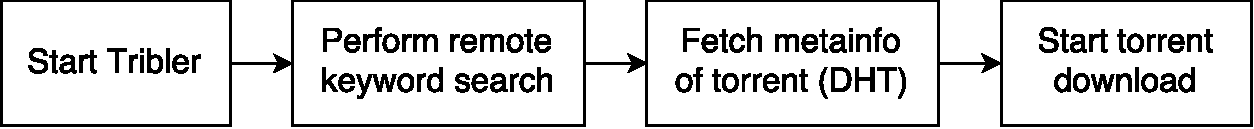
\includegraphics[width=0.7\columnwidth]{images/big_experiment/big_experiment_setup}
	\caption{The actions performed in each run of the experiment described in this Chapter.}
	\label{fig:big-experiment-setup}
\end{figure}

We emphasize that this experiment is performed using the real Tribler network and we are not using an artificial environment. The chosen torrents for the  download operations are random and we are not selecting these torrents based on the health of the swarm.\\\\
We had to implement a workaround for a bug in Tribler: after starting the first anonymous download in Tribler, the download does not receive any bytes. In order to make sure that the download proceeds correctly, we force start the download after the circuits have been established.

\section{Failure Identification}
We can think of various failures during each run of Tribler, both failures on code-level (which should be recognized by the unit tests) and failures that are attributed to external dependencies. Below, we summarize some failures where we abort the Tribler session:
\begin{itemize}
	\item We do not have a sufficient amount of established connections in the \emph{SearchCommunity} after two minutes.
	\item There are no incoming search results after 30 seconds after performing a remote search operation.
	\item We do not receive a response with meta info within 60 seconds after scheduling the five DHT torrent meta info lookup.
	\item Three minutes after the download started, we did not built enough circuits yet.
	\item Three minutes after the download started, we did not receive any content bytes yet.
\end{itemize}
We should not that most of these failures can be addressed to the state of the Tribler network. By performing the run as described in the previous Section many times, we can get insights in the most common failures.

%The order of operations as performed in this experiment is visible in Figure \ref{fig:big-experiment-setup}. The experiment itself is executed on the DAS5 supercomputer where in every run, we allocate ten nodes and run one Tribler instance on every node.\\

%There are various failures that could lead to an interruption of the experiment, which we will summarize below:
%\begin{itemize}
%	\item If we are not connected to at least 30 peers in the \emph{SearchCommunity} after Tribler has started, we abort the experiment.
%	\item If we do not receive any remote torrent result within 30 seconds, we abort the experiment.
%	\item If we do not receive a response from any scheduled DHT lookup, we abort the experiment.
%\end{itemize}
%We also have various failures that influences our result but are not failing our experiment. An example of these failures is when we fail to build circuits within three minutes after starting the download. In this situation, we are still able to finish the experiment, however, our final results are influenced since we were not able to download any byte.

\section{Observed Results}
We will now discuss the results that we obtained during this big, large-scale experiment. The focus will be on the amount and distribution of failures that occurred during the experiment and on the duration of the performed operations.

\subsection{Failure Rates}
After performing the experiments, we observed a success rate of 54.2\% which means that in this percentage of the runs, all operations were successful and that libtorrent downloaded content bytes. In 45.8\% of the runs, we encountered an issue during the Tribler session. The exact distribution of observed failures is presented in Figure \ref{fig:big-experiment-outcome-pie}.

\begin{figure}[!h]
	\centering
	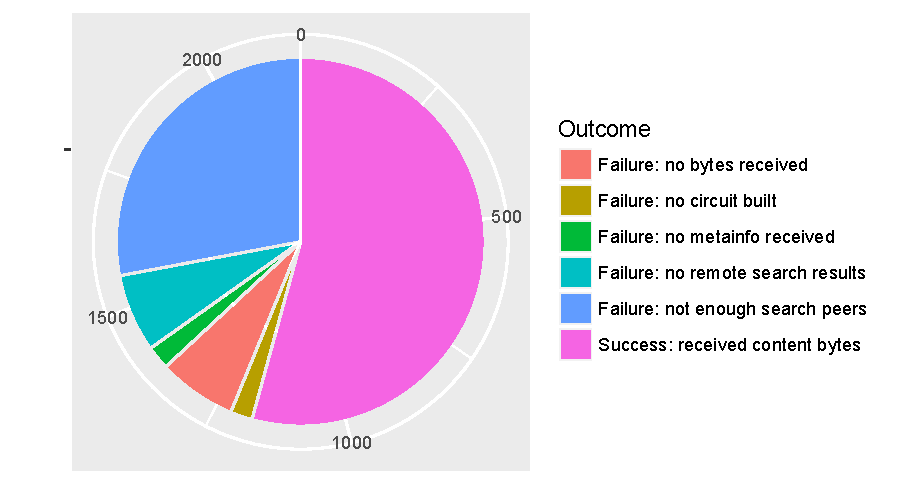
\includegraphics[width=0.7\columnwidth]{images/big_experiment/outcome_pie}
	\caption{The distribution of outcomes of all 2.171 runs.}
	\label{fig:big-experiment-outcome-pie}
\end{figure}

Fortunately, most of the runs are succeeding. However, a significant amount of the failures is addressed to the situation where Tribler did not connect to enough peers in the \emph{SearchCommunity} two minutes after start-up (in 27.9\% of the runs). If this failure occurred during a run, we recorded the amount of peers that are connected after two minutes and we noticed that this amount often between 20 and 30 peers. This indicates that this failure is not significant anymore if we decide to lower the amount of peers required when searching.\\\\
In 6.9\% of the runs, we did not receive any search result after 30 seconds. While this results might contradict our findings in the experiment explained in Chapter \ref{sec:remote-content-search-experiment} where all our queries resulted in at least one search result, we should emphasize that there might be keywords in our constructed query list that have an unevenly distribution amongst peers. In the database we used to construct the query list, we were subscribed on various channels, having access to more content. Peers we are connecting to, might not have discovered many torrents, possibly because they are subscribed to fewer channels. This way, the chance for a peer to contain content matching a specific keyword decreases. Another explanation might be that there is a torrent with many files that contains a rare keyword in a significant part of these files. Our selection algorithm will consider this keyword as common in the database, however, the torrent file might be new where not many peers know about this torrent.\\\\
In 2.1\% of all runs, we did not receive torrent metainfo after scheduling five DHT lookups. In the experiment performed in Section \ref{subsec:dht-experiment}, we found that 48.9\% of the lookups scheduled in the DHT failed. When scheduling five parallel lookups, we estimate that the chance of all requests failing is $ 0.489^5 \approx 0.031 $ or 3.1\%. Of all 2.171 runs, we scheduled the DHT lookups in 1.415 runs. In total, 45 runs failed with an absence of a meta info response, resulting in a percentage of a failure rate of 3.2\% for the DHT lookup operations in our experiment, very close to our expected value. The explanation for the fact that this number is slightly higher might be that we did lookup of more popular torrents in Section \ref{subsec:dht-experiment} whereas we cannot make assumption on the popularity of the torrents we lookup in this experiment.\\\\
In 1.9\% of the runs, we were unable to built any circuits after three minutes. While this number is relatively low, it is an indicator that the circuits building strategy might need some investigation effort to reveal the root cause of this. In 6.9\% of the runs, we received no bytes after circuits have been built, however, this failure might be addressed to the absence of seeders in the network, a factor we cannot easily influence\todo{conclusies hier?}.

\subsection{Experiment Breakdown}
During this experiment, we performed many steps in each run of Tribler and various interesting events are occurring such as the moment when we retrieved search results and the retrieval of the first content bytes during the torrent download. We kept track of the occurrences of these events so we were able to determine the average duration of the operations performed during our experiments. This detailed breakdown is presented in Figure \ref{fig:big-experiment-breakdown} where we show a timeline with various interesting events during the experiment.

\begin{figure}[!h]
	\centering
	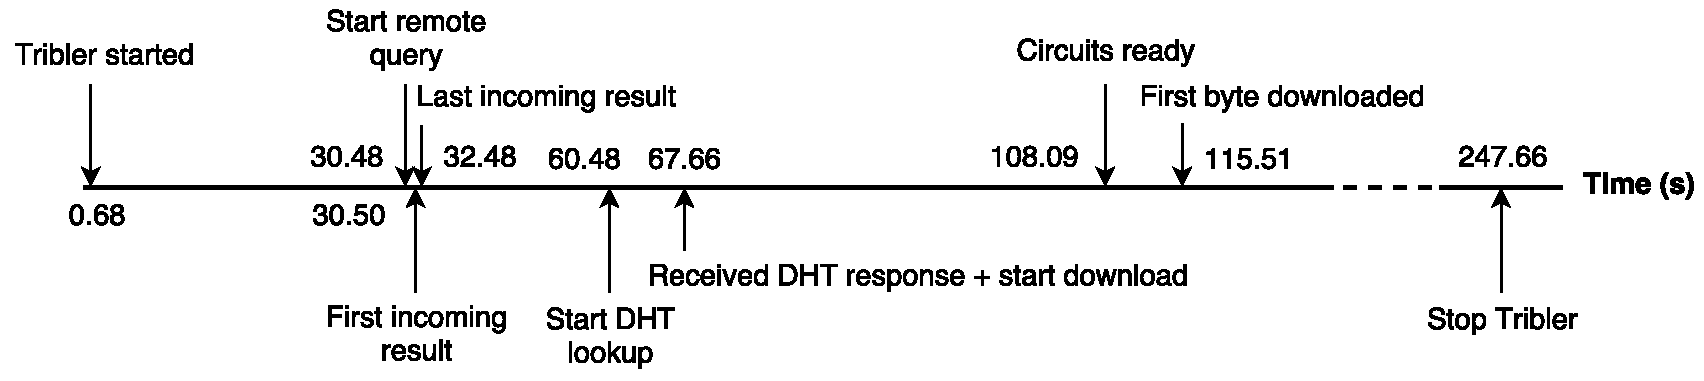
\includegraphics[width=1.0\columnwidth]{images/big_experiment/big_experiment_breakdown}
	\caption{A timeline of interesting events during the runs. All values are averaged.}
	\label{fig:big-experiment-breakdown}
\end{figure}

The average start-up time of Tribler during our experiments is 0.68 seconds. While this is more than the value as determined in Section \ref{sec:startup-experience} (x\todo{welke?}), it is still well under a second. The differences are most likely due to inequality in hardware specifications.\\\\
After around 30 seconds, we have established enough connections to peers in the \emph{SearchCommunity}, after which we perform a remote keyword search. We notice that the first incoming response is fast: on average, it arrives after 20 milliseconds, which is significantly faster than the value determined in Section \ref{sec:remote-content-search-experiment} (260 milliseconds). We believe this is explained due to the faster connection of the DAS5 supercomputer. The last response takes on average around two seconds to arrive, which is comparable to the value determined in \ref{sec:remote-content-search-experiment} (2.1 seconds).\\\\
Exactly 30 seconds after performing our remote search, we schedule our five DHT lookups. On average, it takes 7.16 seconds before our DHT lookup is successful, which is slightly slower than the average lookup time we found during the experiment in Section \ref{subsec:dht-experiment} (5.81 seconds). After we received the first meta info response, we immediately start the download associated to this received meta info.\\\\
After the anonymous download has been started, Tribler attempts to build circuits which takes on average 40.43 seconds which seems a long time if we consider that Tribler has been running for several minutes and we should have a sufficient amount of peers in the community responsible for the management of circuits. To better understand the behaviour of circuit building, we create an ECDF to get an overview of the distribution of time until circuits are ready, see Figure \ref{fig:big-experiment-circuits}.

\begin{figure}[!h]
	\centering
	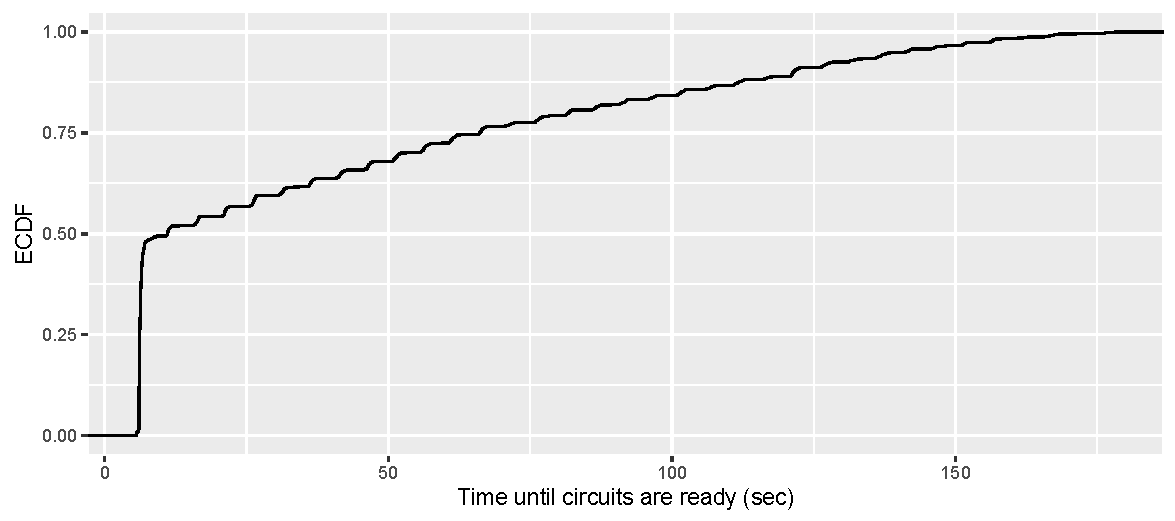
\includegraphics[width=1.0\columnwidth]{images/big_experiment/circuits_ecdf}
	\caption{An ECDF of the time until the circuits are ready.}
	\label{fig:big-experiment-circuits}
\end{figure}

We note that just under 50\% of the circuits are built within 7 seconds. For runs where circuits are taking a longer time to built, we notice a step-like pattern which can be explained by the fact that we are building circuits at fixed time intervals (five seconds). Some circuits can even take several minutes to built. Figure \ref{fig:big-experiment-circuits} shows that the circuit built time can be improved.\\\\
After the circuits are built, it takes on average 7.42 seconds before we received our first byte, which might be slightly but not significantly slower than the time before the first byte is received when performing a non-anonymous download due to our workaround and the overhead of the anonymous overlay network.

\section{Integration in Jenkins}
The experiment described in this Section gave us insights in the failures and duration of various operations in Tribler. In combination with the scenario file mechanism as described in Section \ref{sec:environment-specifications}, we could create a Jenkins job that performs the experiment as described in this Section to give developers feedback about the consequences of their modifications on the operation of core operations. This job can be executed parallel during the testing phase displayed in Figure \ref{fig:jenkins-pipeline}.\\\\
 Due to time constraints, we were not able to implement this feature, however, there are no major technical obstacles for the realisation of this application test.